\section{Работа с контейнерами}

\subsection{Развертывание тестового сервиса внутри контейнера}
\pretolerance10000

В ходе работы по проекту развернут сервис The Hole, взятый с соревнований по информационной безопасности SibirCTF-2018. Под развертыванием сервиса понимается его настройка и запуск внутри контейнера.\par
Для образа контейнера была выбрана операционная система Alpine 3.8. Она была выбрана благодаря небольшому размеру образа и ориентированности на безопасность. Размер чистого образа Alpine с чистого старта 8 Мбайт оперативной памяти в отличии от Ubuntu 16.04 с размером 170 Мбайт. Достигается это за счет минимально необходимого набора системных и прикладных программ. Все дополнительные необходимые программы можно установить с помощью встроенного пакетного менеджера apk.\par
Последовательность действий по развертыванию контейнера:
\begin{itemize}
\item cкачивание образа и создание контейнера с помощью команды lxc launch images:alpine/3.8 sibirctf-hole (рис. 4);
\begin{center}
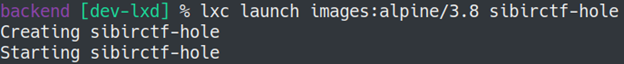
\includegraphics[width=0.65\textwidth]{3}\\
Рисунок 4 -- Результат команды lxc launch\\
\end{center}
\vspace{\baselineskip}

\item подготовка сервиса к загрузке в контейнер;
\item создание сценария командной строки по установке необходимых зависимостей системных и прикладных программ и сборки сервиса: сценарий командной строки по сборке сервиса состоит из установки зависимостей и компиляции исходных кодов сервиса на C++ (рис. 5), сценарий запуска сервиса может состоять из запуска необходимых программ внутри контейнера, но данный сервис не зависит от других программ, поэтому необходимо только выполнить запуск сервиса (рис. 6);
\begin{center}
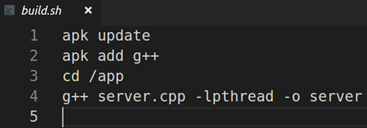
\includegraphics[width=0.45\textwidth]{4}\\
Рисунок 5 -- Сценарий сборки сервиса\\
\end{center}
\vspace{\baselineskip}

\begin{center}
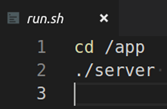
\includegraphics[width=0.3\textwidth]{5}\\
Рисунок 6 -- Сценарий запуска сервиса\\
\end{center}
\vspace{\baselineskip}

\item загрузка подготовленного сервиса в контейнер с помощью команды lxc file push vuln-service-the-hole/* vuln-hole/app/ -p -r -v (рис. 7);
\begin{center}
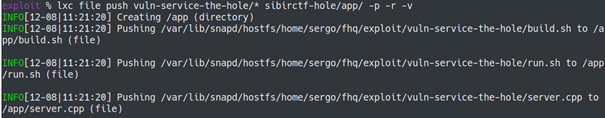
\includegraphics[width=0.65\textwidth]{6}\\
Рисунок 7 -- Загрузка подготовленного сервиса\\
\end{center}
\vspace{\baselineskip}

\item запуск сборки сервиса с помощью команды lxc exec sibirctf-hole sh /app/build.sh (рис. 8);
\begin{center}
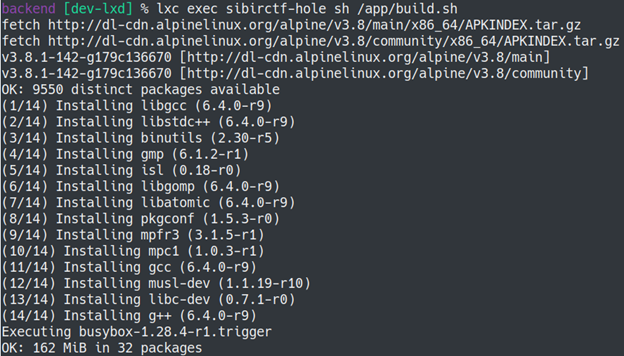
\includegraphics[width=0.65\textwidth]{7}\\
Рисунок 8 -- Сборка сервиса\\
\end{center}
\vspace{\baselineskip}

\item открытие TCP-порта 5003 для доступа к сервису c помощью команды lxc config device add sibirctf-hole port5003 proxy listen=tcp:0.0.0.0:5003 connect=tcp:localhost:5003 (рис. 9);
\begin{center}
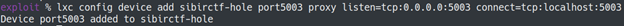
\includegraphics[width=0.8\textwidth]{8}\\
Рисунок 9 -- Открытие порта 5003\\
\end{center}
\vspace{\baselineskip}

\item запуск сервиса внутри контейнера с помощью lxc exec sibirctf-hole sh /app/run.sh (рис. 10);
\begin{center}
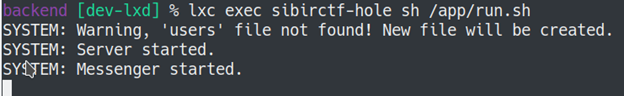
\includegraphics[width=0.65\textwidth]{9}\\
Рисунок 10 -- Запуск сервиса\\
\end{center}
\vspace{\baselineskip}

\item проверка доступа к сервису с локальной машины с помощью nc localhost 5003 (рис. 11);
\begin{center}
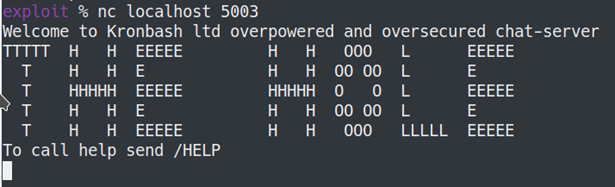
\includegraphics[width=0.65\textwidth]{10}\\
Рисунок 11 -- Проверка доступа к сервису\\
\end{center}

\end{itemize}
\vspace{\baselineskip}

\subsection{Асинхронная обработка запроса операций с контейнером}
В ходе работы над проектом добавлена возможность асинхронно обрабатывать запросы по созданию, запуску, остановке и удалению контейнеров. Необходимо было обрабатывать асинхронные команды LXD, не блокируя основной поток выполнения backend-сервера FreeHackQuest. Рассматривались разные подходы к реализации такие, как feature, promise, task из стандартной библиотеки C++ или сопрограммы из Boost. Но выбран шаблон проектирования пул потоков (Thread Pool) из-за его простоты и достаточности для решения поставленной задачи. Он заранее запускает нужное количество потоков, которые выполняют задачи, поступающие в очередь задач.\par
В ходе работы над задачей возникла проблема отправки сообщения frontend части клиентской стороны -- WebSocket сервер не позволял отправлять сообщение из другого потока. Данную проблему удалось решить с помощью концепции сигналов и слотов. Из потока выполнения задачи в основной поток отправлялся сигнал с сообщением нужному клиенту и в основном потоке слот обрабатывал поступивший сигнал. Тем самым удалось обойти ограничение отправки WebSocket сообщений только из основного потока выполнения.\par
Наглядное представление асинхронной обработки запроса операций с контейнером, а конкретней операция создания контейнера, можно увидеть в виде UML диаграммы последовательности на рисунке 12.
\begin{center}
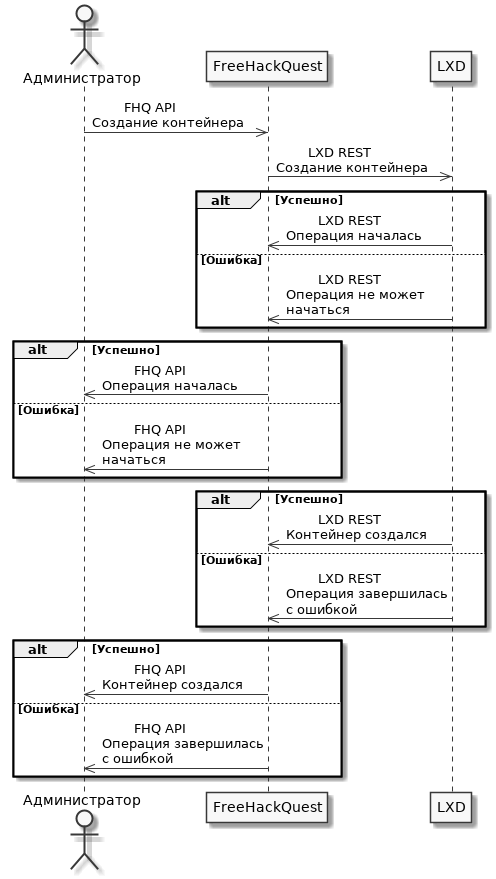
\includegraphics[width=0.65\textwidth]{11}\\
Рисунок 12 -- Асинхронное создание контейнера\\
\end{center}
\vspace{\baselineskip}

\subsection{Настройка подсети-порта для контейнера}
Порты можно настраивать с помощью добавления к контейнеру устройства типа прокси (proxy). Устройство типа прокси позволяет пересылать сетевые соединения между хостом и контейнером. Это позволяет перенаправлять трафик, попадающий на один из адресов хоста, на адрес внутри контейнера. Возможные типы подключения: TCP с TCP, UNIX socket с UNIX socket, TCP с UNIX socket, UDP с UDP и так далее.\par
Открытие TCP порта 5003 для доступа к сервису c помощью команды lxc config device add sibirctf-hole port5003 proxy listen=tcp:0.0.0.0:5003 connect=tcp:localhost:5003 (рис. 13).\par
\begin{center}
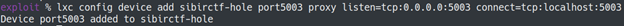
\includegraphics[width=0.8\textwidth]{12}\\
Рисунок 13 -- Открытие порта 5003\\
\end{center}
\vspace{\baselineskip}

Настроить подсеть контейнеров можно с помощью группы команд lxc network. Создать отдельную сеть можно с помощью команды lxc network create <имя\_сети>. Прикрепить созданную сеть к контейнеру можно с помощью команды lxc network attach <имя\_сети> <имя\_контейнера> <имя\_устройства> <имя\_интерфейса>.\par
Настроить использование NAT можно с помощью lxc network set <имя\_сети> ipv4.nat true.\par
Задать IPv4 адрес статически можно с помощью команды lxc config device set sibirctf-hole eth0 ipv4.address 10.105.26.88.\par
После перезагрузки контейнера сетевые адреса обновятся, а команда lxc network list-leases sibirctf покажет наличие записи о статическом адресе для контейнера.\par
 \clearpage